\documentclass{msuappclass}
% Above calls the file msuappclass.cls which provides the "class", or type of document.  This gives a format of the APP according to the Minnesota State University regulations (see http://grad.mnsu.edu/capstone/guidelines.html ).  
\usepackage{msuappstyle}
% Above calls the file msuappstyle.sty file which creates the title page and provides the header and footer settings (mainly to provide the page number in the upper right corner of each page).  It also calls on all of the style files that you should need for the math symbols, etc.


\usepackage{amscd}
\usepackage{amsmath}
%\usepackage{graphics}
\usepackage[rightcaption]{sidecap}
%\usepackage{setspace}
%\usepackage[author-year]{amsrefs}

\usepackage{tikz}
\usetikzlibrary{arrows}


\theoremstyle{theorem}
\newtheorem{theorem}{Theorem}[chapter]
\newtheorem{definition}{Definition}
\newtheorem{example}{Example}[section]


\newcommand{\reals}{\mathbb{R}}
\newcommand{\rats}{\mathbb{Q}}
\newcommand{\nats}{\mathbb{N}}
\newcommand{\ints}{\mathbb{Z}}
\newcommand{\ra}{\rightarrow}
\newcommand{\ds}{\displaystyle}
\newcommand{\invlim}[2]{\underleftarrow{Lim}(#1, #2)}
\newcommand{\drctlim}[2]{\varinjlim{(#1,#2)}}   %$\drctlim{a}{b}$

\begin{document}

% \pagenumber{roman} numbers the pages in roman style: i, ii, etc.   
\pagenumbering{roman}

%  \apptitle calls on a command created in the style file "msuapp".  This file handles much of the formatting of the paper, and also builds the title page of the APP.  The first field is the name of the paper.  Second field is your name.  Third field is Master of Arts or Master of Sciences.  Last field is the date you will graduate.

\apptitle
	{\sc Title}
	{Your name}
	{thesis} %thesis (or) dissertation (or) alternative plan paper    
	{Master of Arts}
	{Information Technology} %Name of your degree
	{Month Year}

\thispagestyle{empty}

\begin{flushright}
May, 2010
\end{flushright}

\noindent This [thesis (or) dissertation (or) Alternate Plan Paper] has been examined and approved  by the following members of the student's committee: \\

  
%\noindent Examining Committee:

\hspace{3in}\underline{\hspace{2.5in}}

\hspace{3in}Dr. Brian Martensen, Chairperson

\vspace{0.5in}
\hspace{3in}\underline{\hspace{2.5in}}

\hspace{3in}Dr. Charles Waters

\vspace{0.5in}
\hspace{3in}\underline{\hspace{2.5in}}

\hspace{3in}Dr. Michael Spencer


%\thispagestyle{empty}

\begin{center}
\large  Abstract
\end{center}




\renewcommand{\baselinestretch}{0.1}


%\begin{singlespace}
Lorem ipsum dolor sit amet, consectetur adipiscing elit, sed do eiusmod tempor incididunt ut labore et dolore magna aliqua. Ut enim ad minim veniam, quis nostrud exercitation ullamco laboris nisi ut aliquip ex ea commodo consequat. Duis aute irure dolor in reprehenderit in voluptate velit esse cillum dolore eu fugiat nulla pariatur. Excepteur sint occaecat cupidatat non proident, sunt in culpa qui officia deserunt mollit anim id est laborum.

%\end{singlespace}



\renewcommand{\baselinestretch}{\spacing}

% These are the possible sections of your paper.  I didn't use the parts that have been percentaged, but you can unpercentage them if needed.  Anything that should be before "Page 1", should be included before "\pagenumbering{arabic}".

%\include{ack}\
\tableofcontents
\listoffigures
\thispagestyle{empty}

\begin{center}
\large  Abstract
\end{center}




\renewcommand{\baselinestretch}{0.1}


%\begin{singlespace}
Lorem ipsum dolor sit amet, consectetur adipiscing elit, sed do eiusmod tempor incididunt ut labore et dolore magna aliqua. Ut enim ad minim veniam, quis nostrud exercitation ullamco laboris nisi ut aliquip ex ea commodo consequat. Duis aute irure dolor in reprehenderit in voluptate velit esse cillum dolore eu fugiat nulla pariatur. Excepteur sint occaecat cupidatat non proident, sunt in culpa qui officia deserunt mollit anim id est laborum.

%\end{singlespace}



\renewcommand{\baselinestretch}{\spacing}

% \pagenumber{arabic} restarts the numbering and numbers the pages at 1.


 \chapter{\sc Introduction}



\section{daf}
	\subsection{asdf}


$\displaystyle{\sum_{i=0}^n i = \dfrac{n(n+1)}{2} \mathcal{O}(n^2) }$

In this paper we are interested in determining if two aperiodic tilings are essentially different (combinatorially).  Here, aperiodic  means no translation of the tiling produces the original tiling.  Aperiodic tilings have a long history.  For a more complete account see Sadun's \textit{Topology of Tiling Spaces} \cite{sad} or Radin's \textit{Miles of Tiles} \cite{radin-2}. In the 1960's, Hao Wang \cite{wang} studied tilings in relation to decidability problems.  He proposed the Domino Problem concerning whether the plane could be tiled using Wang Dominoes.  Robert Berger \cite{berg} showed this problem was undecidable, which immediately implies the existence of an aperiodic tiling.  In this proof, he constructed a 20,426 wang tile example.
It has been studied by many since then, and in 1974, Roger Penrose \cite{pen} reduced the number of prototiles required to only two, with the Kites and Darts tiling, Figure~\ref{fig:example}.   Substitutions provide straightforward ways to produce aperiodic tilings.  As such, many examples are known.  It is an open problem, referred to as the Einstein problem, to construct an periodic tiling with one prototile.  The pinwheel tiling, as suggested by John Conway and constructed by Charles Radin, is constructed with a single tile, in that it uses a single shape, but one must use this tile in infinitely many orientations, along with their reflections. 

\begin{figure}[htbp] %  figure placement: here, top, bottom, or page
   \centering
   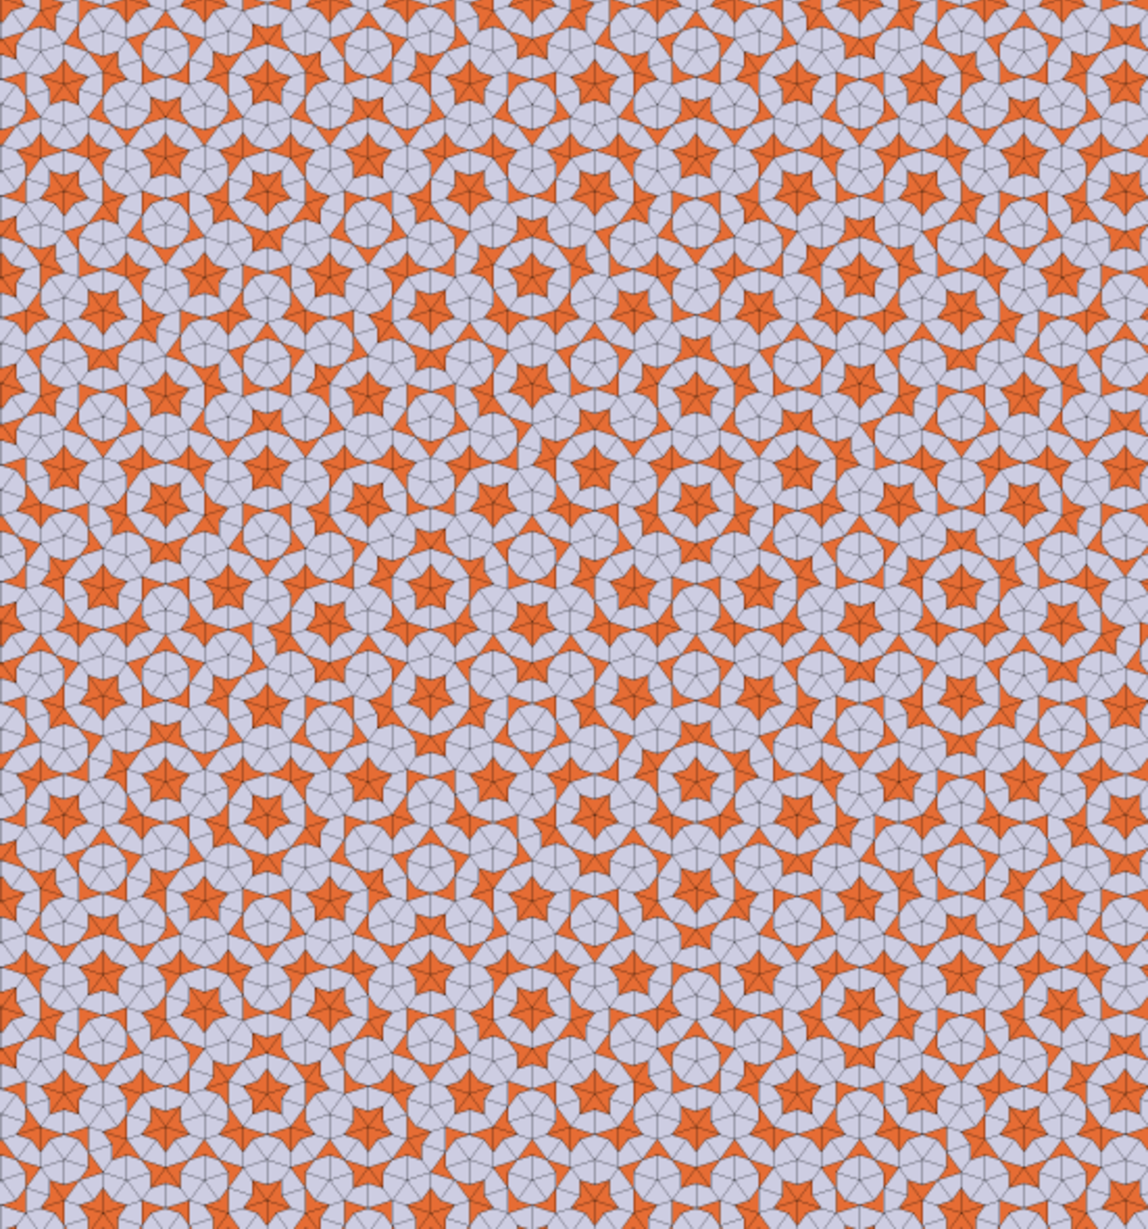
\includegraphics[width=2.5in]{./figs/penrose.pdf} 
   \caption{Penrose kite and dart tiling from the Tilings Encyclopedia Website (\texttt{http://tilings.math.uni-bielefeld.de/substitution$\empty\_$rules/})}
   \label{fig:example}
\end{figure}


\pagenumbering{arabic}

\chapter{\sc Constructing Tiling Spaces}

We have different methods of constructing tiling spaces.  The first is to be generated by a set of tilings.  If we take $\reals^n$ and subdivide it into different pieces, then each individual piece is called a $\mathit{tile}$, where each tile overlaps another only at its border.  The union of all the tiles is called a $\mathit{tiling}$. For our examples we will only have a finite number of tile types, up to translation, called prototiles.  Each prototile is a polytope.  For a simple example let $n=1$, and let  $T= \cup_{i\in \ints} \ t_i$, where $t_i = [i, i+1]$.  Then each tile only intersects another tile at its boundary points and $T=\cup \ t_i = \reals$.
 A $\mathit{translation}$ of a tiling T is a shift of the tiling by some vector $x\in \reals^n$.  Let T be as above, then $T-1$ is a translation of T to the right by one unit.  
 
 We can place a metric on tilings by considering two tilings close (within $\epsilon$) if after a small translation ($\epsilon$) these tiles agree on a large radius (1/$\epsilon$) about the origin.  It is difficult to state the metric formally.  In the following definition, the closure and therefore, the topology, is given by this metric.
 
 \begin{definition}
 A tiling space $\Omega_T$ is a set of tilings that has the following two properties
 \\ \indent 1) For each $T \in \Omega_T$ and each $x \in \reals^n$ implies $T-x \in$ $\Omega_T$
 \\ \indent 2) $\overline{ \{ T-x \ | \  x \in \reals^n \} }  \subseteq  \Omega_T$ for each T $\in \Omega_T$
 
 \end{definition}
 



 
% \include{figures}
 %\include{app1}
  %\include{footnotes}


\bibliography{ref.bib}

\bibliographystyle{amsalpha}

\end{document}
